\chapter{Cvičení 3}
\section{Střední hodnota náhodné veličiny}
Střední hodnota označuje míru polohy a středu hustoty pravděpodobnosti náhodné veličiny (další míry polohy jsou například modus a medián). Střední hodnota je definována jako integrál funkce vzhledem k nějaké pravděpodobnostní míře.

\begin{enumerate}[noitemsep, label=\alph*)]
	\item \textbf{Lebesgueův integrál} vzhledem k abstraktnímu pravděpodobnostnímu prostoru $\{\Omega,\mathscr{F},P\}$ je
	\[ E[X] \triangleq \int\limits_\Omega X(\omega)\d P(\omega) \]
	
	\item \textbf{Riemanův-Stieltjesův} integrál na $\{\mathbb{R}, \mathscr{B}(\mathbb{R}), F_x(x)\}$ ve tvaru
	\[ E[X] = \int\limits_{-\infty}^\infty x\d F-x(x) \]
	
	\item \textbf{Riemanův} integrá, dokud je $F_x(x)$ diferencovatelná $\d F_x(x)$ je roven hustotě pravděpodobnosti $p_x(x)\d x$, pak
	\[ E[X] = \int\limits_{-\infty}^\infty x p_x(x)\d x \]
\end{enumerate}

	\subsubsection{Riemanova suma}
	\[ R(N) = \sum_{n=1}^N g(\alpha_n)(x_{n-1}-x_n),\]
	
	kde $\alpha_n$ je nějaký bod intervalu $\langle x_n, x_{n+1}\rangle$.
	
	\begin{figure}
	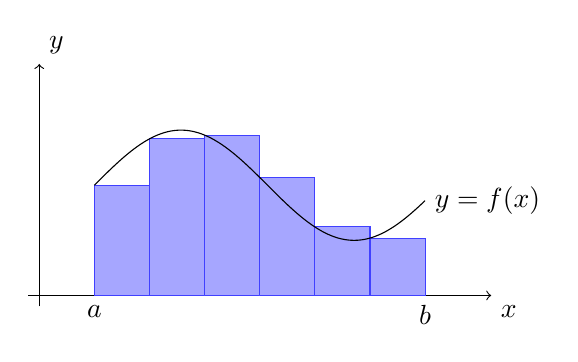
\begin{tikzpicture}[scale =.7]
    \draw[->] (-.2,0) -- (8.2,0) node[below right] {$x$};
    \draw[->] (0,-.2) -- (0,4.2) node[above right] {$y$};
 
    \foreach \x in {0,1,...,5} {
      \draw[fill=blue!35, draw=blue!75] (\x + 1,0) -- ++(1,0) -- ++(0,{sin(\x r) ++ 2}) --
      ++(-1,0) -- ++(0,{-sin(\x r) - 2});
    }
 
    \draw[domain=0:6,samples=100] plot(\x + 1,{sin(\x r) + 2})
    node[right] {$y = f(x)$};
 
    \draw (1,0) node[below] {$a$};
    \draw (7,0) node[below] {$b$};
	\end{tikzpicture}
	\end{figure}
	
	\subsubsection*{Riemanův-Stieltjesova suma}
	\[ RS(N) = \sum_{n=1}^N g(\alpha_n)(h(x_{n-1})-h(x_n)),\]
	
	kde $h(\cdot)$ je neklesající funkce.
	
	\subsubsection*{Lebesgueůvova suma}
	\[ LB(N) = \sum_{n=1}^N g_n\cdot L(x\in\langle a, b\rangle, y_n\leq g(x)<y_{n+1})\]
	
	\subsection{Dirichletova funkce}
	Tato funkce není spojitá v žádném bodě,  není monotónní v žádném bodě a v žádném bodě nemá limitu. Nabývá dvou hodnot 0 a 1, kde
	\[ D(x) =
	\begin{cases}
	0 & \text{$x$ je iracionální číslo}\\
	1 & \text{$x$ je racionální číslo}
	\end{cases}
	\]
	
	\begin{eqnarray*}
	LB(N) &=& \sum_{n=1}^N y_n\cdot L(x\in\langle a, b\rangle, y_n\leq g(x)<y_{n+1})=\\
	&=& 0 L(x\in\langle a, b\rangle, 0\leq g(x)<1) + 1 L(x\in\langle a, b\rangle, 0\leq g(x)<\infty) = L(\mathbb{Q})=0
	\end{eqnarray*}
	
	\begin{note}{Příklad}
	Házení 2 mincemi, $\Omega=\{PP,PO,OP,OO\}$,\\$\mathscr{A}=\{\emptyset, \Omega, \{PP,OO\},\{PO\},\{OP\},\{PO,OP\},\{PP,OP,OO\}, \{PP,OO,PO\}\}$.a $X(\omega)=I_{\{PP,OO\}}(\omega)$. Střední hodnota $E[X(\omega)]$ se vypočte jako
	
	\begin{eqnarray*}
	E[X(\omega)] &=& \int\limits_\Omega X(\omega)\d P(\omega)=\\
	& = & 1\cdot P(\omega\in\Omega, x(\omega)=1) + 0\cdot P(\omega\in\Omega, x(\omega)=0)=\\
	& = & 1\cdot P(\{OO,PP\}) + 0\cdot P(\{OP,PO\}) = \frac{1}{4}+\frac{1}{4} = \frac{1}{2}
	\end{eqnarray*}
	\end{note}
	
	\begin{note}{Příklad}
		$x$ má normální rozložení s parametry $\mu,\sigma^2$, pro které je střední hodnota
		\[ E[X] = \int\limits_{-\infty}^\infty xp_x(x)\d x= \int\limits_{-\infty}^\infty x\frac{1}{\sqrt{2\pi\sigma^2}}e^{-\frac{1}{2}\frac{(x-\mu)^2}{\sigma^2}}\d x=\mu \]
		
		\[ \int\limits_{-\infty}^\infty (x-\mu)\frac{1}{\sqrt{2\pi\sigma^2}}e^{-\frac{1}{2}\frac{(x-\mu)^2}{\sigma^2}}\d x = 0 \]
		
		\[ \int\limits_{-\infty}^\infty x\frac{1}{(\cdot)}e^{-\frac{1}{2}(\cdot)}\d x = \int \mu\frac{1}{(\cdot)}e^{-\frac{1}{2}(\cdot)}\d x = \mu\int\limits_{-\infty}^\infty \frac{1}{(\cdot)}e^{-\frac{1}{2}(\cdot)}\d x = \mu \]
		
		$x$ má Cauchyho rozdělení s parametrem $C=0$. Pravděpodobnost $P$ je 
		\[ p_x(x) = \frac{\frac{\alpha}{\pi}}{x^2 + \alpha^2} \]
		
		Střední hodnotu Cauchyho rozdělení spočteme tedy jako
		\[ E[X] = \int\limits_{-\infty}^\infty x\frac{\frac{\alpha}{\pi}}{x^2 + \alpha^2}\d x = \frac{\alpha}{2\pi}\int\limits_{-\infty}^\infty \frac{2x}{x^2 + \alpha^2}\d x = \frac{\alpha}{2\pi}\left[ \ln(x^2+\alpha^2) \right]_{-\infty}^\infty = "\infty-\infty" \]
		
		Z výsledku plyne, že střední hodnota Cauchyho rozdělení \textbf{neexistuje}.
		
		\begin{figure}
		\begin{tikzpicture}[scale=.7]
		\begin{axis}[every axis plot post/.append style={
  mark=none,domain=-2:3, y domain = 0:1, samples=50,smooth}, % All plots: from -2:2, 50 samples, smooth, no marks
  axis x line*=bottom, % no box around the plot, only x and y axis
  axis y line*=left, % the * suppresses the arrow tips
  enlargelimits=upper,ymin = 0] % extend the axes a bit to the right and top
  \addplot {gauss(1,0.75)*2};
  \addplot {(x-1)/2};
\end{axis}
		\end{tikzpicture}
		\end{figure}
	\end{note}
	
	\subsection{Vlastnosti střední hodnoty}
	Pro pravděpodobnost
	\begin{eqnarray*}
	P(a\leq x \leq b) & = & E[I_{\langle a,b\rangle}(x)] = \\
	& = & \int\limits_{-\infty}^\infty I_{\langle a,b\rangle}(x)p_x(x)\d x = \\
	& = & \int\limits_a^b p_x(x)\d x = F_x(b)-F_x(a)
	\end{eqnarray*}
	
	Jako jedna z nejdůležitějších vlastností střední hodnoty je \textbf{linearita}, která dokazuje, že střední hodnota $E[X]$ je lineární operátor
	\[ E[aX+bY] = aE[X] + bE[Y], \]
	
	kde koeficienty $a,b$ jsou konstanty a $X,Y$ náhodné veličiny. Další důležitou vlastností střední hodnoty je \textbf{nezávislost}, která definuje případ, kdy jsou $\{X_1,X_2,\ldots, X_n\}$ nezávislé. Zde platí střední hodnota
	\[ E[X_1,X_2,\ldots,X_n]=\prod_{n=1}^N E[X_n] \]
	
	Pro dvě náhodné veličiny $X$ a $Y$ tedy platí
	\[ E[X\cdot Y] = \iint X\cdot Y p_{x,y}(x,y)\d x\d y = \int Xp_x\d x\int Y p_y\d y \]
	
	\subsection{Vlastnosti podmíněné střední hodnoty}
	Podmíněnou střední hodnotu, tj. střední hodnotu jevu $X$ za podmínky, že nastal jev $Y$, spočteme jako
	\[ E[X|Y=y]\triangleq \int x p_{X|Y}(x|y)\d x = f(y), \]
	
	kde $f(y)$ zde značí funkci a víme, jak dopadlo $Y$. Podmíněnou střední hodnotu pro náhodnou veličinu pak zapisujeme jako
	\[ E[X|Y]\triangleq x p_{X|Y}(x|y)\d x = \gamma(Y), \]
	
	přičemž $\gamma$ značí gamma funkci a nevíme, jak dopadlo $Y$.
	
	\subsection{Věta o úplné střední hodnotě}
	Jelikož střední hodnota je lineární operátor, můžeme výraz $E[X]=E[E[X|Y]]$ zapsat jako
	
	\begin{eqnarray*}
	\int\left[\int xp(x|y)\d x\right]p(y)\d y & = & \iint xp(x,y)\d x\d y = \\
	& = & \int x\left(\int p(x,y)\d y\right)\d x =\\
	& = & \int x p(x)\d x = E[x]
	\end{eqnarray*}
	
	\begin{note}{Příklad}
	Nejprve házíme kostko a poté mincí tolikrát, kolik padne ok na kostce. Jev $X$ značí počet \textbf{orlů}, které padnou na minci a jev $Y$ počet \textbf{ok} na kostce. Střední hodnoty jevu $Y$ mohou být například
	
	\begin{eqnarray*}
		E[X|Y=1] & = & \frac{1}{2}\\
		E[X|Y=2] & = & 1\\
		&\vdots &\\
		E[X|Y=6] & = & 3
	\end{eqnarray*}
	
	Obecně tam můžeme tuto střední hodnotu zapsat jako
	\[ E[X|Y] = \frac{Y}{2} \]
	
	Přičemž střední hodnotu složeného výrazu vypočítáme
	\begin{eqnarray*}
	E[X] & = & E[E[X|Y]]=E\left[\frac{1}{2}\right] = \frac{1}{2}E[Y] =\\
	& = & \frac{1}{2}\cdot\frac{21}{6}=\frac{7}{4}
	\end{eqnarray*}
	
	\end{note}